%
% slides.tex
%
% (c) 2019 Prof Dr Andreas Müller, Hochschule Rapperswil
%

\begin{document}

\theoremstyle{definition}
\newtheorem{signal}{Signal}
\newtheorem{abgetastet}{Abgetastetes Signal}
\newtheorem{skalar}{Skalarprodukt und Norm}
\newtheorem{cauchyschwarz}{Cauchy-Schwarz-Ungleichung}
\newtheorem{nachteile}{Nachteile}
\newtheorem{idee}{Idee}
\newtheorem{faktoren}{Erfolgsfaktoren}

\ifthenelse{\boolean{presentation}}{
\begin{frame}
\titlepage
\end{frame}
}{}

%
% Vergleich von Funktionen
%
\def\vergleich#1{
\begin{frame}
\frametitle{Funktionsvergleich}
\centering
\includegraphics[width=\hsize]{#1}
\end{frame}
}

\vergleich{../../buch/chapters/1-geometrie/images/sinsin.pdf}
\vergleich{../../buch/chapters/1-geometrie/images/sincos.pdf}
\vergleich{../../buch/chapters/1-geometrie/images/sinrect.pdf}
\vergleich{../../buch/chapters/1-geometrie/images/cosrect.pdf}
\vergleich{../../buch/chapters/1-geometrie/images/sinrand.pdf}

\begin{frame}
\frametitle{Skalarprodukt von abgetasteten Signalen}
\begin{signal}
Funktion $\mathbb R \to \mathbb R$:
\[
t\mapsto f(t)
\]
\end{signal}

Abtastung: Auswertung an Stellen $t_k = hk$, $h=\text{Abtastinterval}$,
$k\in\mathbb Z$, ergibt $f_k=f(t_k)$

\begin{abgetastet}
Funktion $\mathbb Z\to \mathbb R: k\mapsto f_k $
\end{abgetastet}

\begin{skalar}
Mass für Ähnlichkeit:
\[
\langle x,y\rangle
=
\langle x_k, y_k \rangle
=
\sum_{k\in\mathbb Z} x_ky_k
\qquad
\|x\|^2 = \langle x,x\rangle = \sum_{k\in\mathbb Z} |x_k|^2
\]
\end{skalar}

\end{frame}

%
% Geometrische Intuition für das Skalarprodukt
%
\begin{frame}
\frametitle{Geometrie}
\begin{cauchyschwarz}
\[
|\langle x,y\rangle| \le \langle x,x\rangle \cdot \langle y,y\rangle
= \|x\|\cdot \|y\|
\]
Gleichheit genau dann, wenn $x$ und $y$ linear abhängig sind.
\end{cauchyschwarz}
Masszahl für ``Ähnlichkeit'' von Signalen:
\[
-1 \le \frac{\langle x,y\rangle}{\|x\|\cdot \|y\|}\le 1
\]
\begin{itemize}
\item
Nahe bei $\pm 1$: ähnlich
\item
Gleichheit genau dann, wenn $x$ und $y$ Vielfache voneinander
\end{itemize}
$\Rightarrow$ Vektorgeometrie für Signale, Orthonormalbasis
\end{frame}

%
% Fourier-Idee
%
\begin{frame}
\frametitle{Fourier-Idee}
\begin{idee}
Vergleich mit $\sin(\omega t)$ und $\cos(\omega t)$ für beliebige Frequenzen
$\omega\in\mathbb R$.
\end{idee}
\bigskip

Fourier-Koeffizienten:
\[
\langle \sin(\omega t), f(t) \rangle
\qquad\text{und}\qquad
\langle \cos(\omega t), f(t) \rangle
\]

\bigskip

\begin{nachteile}
\begin{enumerate}
\item
$\sin(t + 2\pi) = \sin(t)$
$\Rightarrow$ 
das um $2\pi$ zeitverschobene Signal liefert den gleichen
Fourier-Koeffizienten
\item
Fourierkoeffizient $\langle \sin t, f\rangle$ sagt nichts darüber aus, wo
$f$ ``interessant'' ist
\item
Fourier-Transformation kann erst bestimmt werden, wenn das ganze Signal
``vorbei'' ist.
\end{enumerate}
\end{nachteile}
\end{frame}

%
% Wavelet-Idee
%
\begin{frame}
\frametitle{Wavelet-Idee}
\begin{idee}
Signal vergleichen mit kurzen Wellenstückchen: ``Wavelets''
\end{idee}
\begin{faktoren}
\begin{itemize}
\item 
``Gute'' Wavelets, vergleichbar mit realistischen Signalen
$\rightarrow$
Mexikanerhut, Meyer-Wavelet, Gabor-Wavelet, Daubechies-Wavelets, Coifflet,
Symmlet, 
\item 
Schneller Berechnungsalgorithmus
$\rightarrow$
Multiskalen-Analyse,
Wavelets mit kompaktem Träger
\item 
Schneller Synthesealgorithmus
\item 
orthonormierte Basis
$\rightarrow$ Frame, Multiskalen-Analyse
\end{itemize}
\end{faktoren}
\end{frame}

%
% Stueckweise konstante Funktionen
%
\def\stueck#1{
\begin{frame}
\frametitle{Stückweise konstante Funktionen}
\centering
\includegraphics[width=\hsize]{#1}
\end{frame}
}

\stueck{../../buch/chapters/3-haar/images/stueckweise1.pdf}
\stueck{../../buch/chapters/3-haar/images/stueckweise8.pdf}
\stueck{../../buch/chapters/3-haar/images/stueckweise64.pdf}

%
% Haar-Vaterwavelet
%
\begin{frame}
\frametitle{Haar-Vater-Wavelet}
\centering
\begin{tikzpicture}[>=latex]

\only<1>{
\node at (2,1) [above] {$\varphi$};
\fill[color=blue!10] (0,0)--(4,0)--(4,1)--(0,1)--cycle;
\draw[line width=1pt,color=blue] (-0.1,0)--(0,0);
\draw[line width=0.1pt,color=blue] (0,0)--(0,1);
\draw[line width=1pt,color=blue] (0,1)--(4,1);
\draw[line width=0.1pt,color=blue] (4,0)--(4,1);
\draw[line width=1pt,color=blue] (4,0)--(12.1,0);
}
\only<2>{
\node at (6,1) [above] {$T_1\varphi$};
\fill[color=blue!10] (4,0)--(8,0)--(8,1)--(4,1)--cycle;
\draw[line width=1pt,color=blue] (-0.1,0)--(4,0);
\draw[line width=0.1pt,color=blue] (4,0)--(4,1);
\draw[line width=1pt,color=blue] (4,1)--(8,1);
\draw[line width=0.1pt,color=blue] (8,0)--(8,1);
\draw[line width=1pt,color=blue] (8,0)--(12.1,0);
}
\only<3>{
\node at (10,1) [above] {$T_2\varphi$};
\fill[color=blue!10] (8,0)--(12,0)--(12,1)--(8,1)--cycle;
\draw[line width=1pt,color=blue] (-0.1,0)--(8,0);
\draw[line width=0.1pt,color=blue] (8,0)--(8,1);
\draw[line width=1pt,color=blue] (8,1)--(12,1);
\draw[line width=0.1pt,color=blue] (12,0)--(12,1);
\draw[line width=1pt,color=blue] (12,0)--(12.1,0);
}
\only<4>{
\node at (1,{sqrt(2)}) [above] {$D_{\frac12}\varphi$};
\fill[color=blue!10] (0,0)--(2,0)--(2,{sqrt(2)})--(0,{sqrt(2)})--cycle;
\draw[line width=1pt,color=blue] (-0.1,0)--(0,0);
\draw[line width=0.1pt,color=blue] (0,0)--(0,{sqrt(2)});
\draw[line width=1pt,color=blue] (0,{sqrt(2)})--(2,{sqrt(2)});
\draw[line width=0.1pt,color=blue] (2,0)--(2,{sqrt(2)});
\draw[line width=1pt,color=blue] (2,0)--(12.1,0);
}
\only<5>{
\node at (0.5,{2}) [above] {$D_{\frac12}\varphi$};
\fill[color=blue!10] (0,0)--(1,0)--(1,{2})--(0,{2})--cycle;
\draw[line width=1pt,color=blue] (-0.1,0)--(0,0);
\draw[line width=0.1pt,color=blue] (0,0)--(0,{2});
\draw[line width=1pt,color=blue] (0,{2})--(1,{2});
\draw[line width=0.1pt,color=blue] (1,0)--(1,{2});
\draw[line width=1pt,color=blue] (1,0)--(12.1,0);
}

\draw[->,line width=0.7pt] (-0.1,0)--(12.4,0) coordinate[label={$t$}];
\draw[->,line width=0.7pt] (0,-0.1)--(0,2.3) coordinate[label={left:$\varphi$}];

\foreach \x in {1,...,3}{
	\draw[line width=0.7pt] ({4*\x},-0.1)--({4*\x},0.1);
	\node at ({4*\x},-0.1) [below] {$\x$};
}

\end{tikzpicture}
\end{frame}

%
% Themenplan
%
\begin{frame}
\frametitle{Themenplan}
\centering
\begin{tabular}{rp{12cm}}
18. 2.&Einführung\\
25. 2.&Komplexe Zahlen, Fourier-Theorie\\
 4. 3.&Frames: orthonormierte Basen, Frames, Rekonstruktion mit Frames\\
11. 3.&Stetige Wavelet-Transformation: Vorläufer (Fourier, Gefensterte FT),
       Lokalisierung, Skalierung und Translation\\
18. 3.&Rekonstruktionsformel und Zulässigkeitsbedingung für Wavelets\\
25. 3.&Multiskalen-Analyse: $V$, $W$, Projektionen, $\varphi$ und $\psi$\\
 1. 4.&Konstruktion des Mutter-Wavelets: erzeugende Funktion $H(\omega)$,
       Funktionalgleichung für $\varphi$, Definition von $\psi$\\
 8. 4.&Schnelle Wavelet-Transformation und Filterbänke\\
15. 4.&Daubechies-Wavelets\\
{\color{gray}22. 4.}&\text{\color{gray}Ostermontag}\\
{\color{gray}29. 4.}&\text{\color{gray}Reserve/Arbeitssitzung}\\
6. 5.&Beginn Vorträge\\
{\color{red}25. 5.}&\text{\color{red}Abschluss-Sitzung}\\
\end{tabular}
\end{frame}

\end{document}
